% displayname : Physique du laser
\documentclass[12pt,fancy]{cours}
\Chapit{3}{5}
\begin{document}
\maketitre[***]{
  Dans ce dernier chapitre, nous expliquons le principe de fonctionnement d'un laser. Nous présentons les processus d'interaction lumière-matière à l'œuvre dans une cavité laser, et expliquons comment l'émission stimulée permet de produire et d'amplifier un faisceau lumineux cohérent. Nous étudions aussi les propriétés géométriques du faisceau laser.
  }{
\item 
% \item Document de cours Statique des fluides - 2
% \item TD Signaux 2
}



%%%%%%%%%%%%%%%%%%%%%%%%%%%%%%%%%%%%%%%%%%%%%%%%%%%%%%%%%%%%%%%%%%%%%%%
\section{Généralités}

% \subsection{Principe d'un laser}
Avant de devenir le nom commun \guill{laser}, le terme LASER était l'acronyme de l'expression anglaise \emph{Light Amplification by Stimulated  Emission of Radiation}, que l'on peut traduire par \emph{amplification de la lumière par émission stimulée de rayonnement}. Le processus d'émission stimulée, qui est au cœur du fonctionnement du laser, et qui sera étudié en \Sec{stimu}, est responsable de propriétés remarquables du faisceau laser, à savoir :
\begin{liste}
  \item son excellente \imp{cohérence} : le faisceau laser est constitué d'une onde électromagnétique quasi-monochromatique, dont la longueur de cohérence temporelle peut atteindre plusieurs kilomètres pour les lasers les plus performants ;
  \item son excellente \imp{directivité} : le faisceau laser est très peu divergent, et peut être focalisé sur une tache de quelques micromètres de diamètre à plusieurs mètres de distance ;
\end{liste}
Les premières recherches sur le processus d'émission stimulée ont permis l'invention du MASER en 1954 par C. \textsc{Townes} et A. \textsc{Schawlow},
ancêtre du laser dont la fréquence d'émission se situe dans le domaine des micro-ondes. Le laser fut inventé peu de temps après en 1960 par T. \textsc{Maiman}. La plupart des lasers se compose essentiellement de trois éléments :
\begin{enumerate}
  \item un \imp{milieu amplificateur} : il s'agit du milieu dans lequel se produit l'émission stimulée  à l'origine de l'amplification lumineuse. Les milieux peuvent être solides (cristaux ou verres dopés), liquides (colorants organiques), ou gazeux (gaz rares, molécules diatomiques, etc.) ;
  \item une \imp{cavité optique} : il s'agit d'un ensemble de deux miroirs placés en regard entre lesquels le faisceau laser effectue un grand nombre d'aller-retours, ce qui permet d'augmenter son intensité et de sélectionner une raie très fine du spectre d'émission du laser. La cavité joue en somme le rôle d'un interféromètre de Fabry-Pérot ;
  \item un système de \imp{pompage optique} : il s'agit d'une source d'énergie destinée à exciter le milieu amplificateur afin de créer une inversion de population nécessaire à l'amplification lumineuse. Le pompage optique peut être réalisé par une lampe flash (laser impulsionnel), une décharge électrique (laser à gaz), ou un autre laser.
\end{enumerate}

\begin{remarque}
  Les diodes laser, aussi appelées \emph{lasers à semi-conducteurs}, fonctionnent sur un principe différent. Leur fonctionnement est fondé sur la recombinaison radiative de porteurs de charge dans une jonction PN, qui ne fait pas appel au processus d'émission stimulée, et ce sans nécessité de pompage optique, ni de cavité optique.
\end{remarque}


\begin{fig}[laser_schema]
  \centering
  
\includegraphics[scale=1]{laser_schema.pdf}
  \capt{Schéma de principe d'un laser. Le milieu amplificateur est placé entre deux miroirs sphériques, l'un totalement réfléchissant, l'autre partiellement réfléchissant. Le système de pompage optique permet de créer une inversion de population dans le milieu amplificateur. Le faisceau laser sortant est un faisceau gaussien très peu divergent.}
\end{fig}

Les deux premiers lasers inventés furent les suivants.
\begin{liste}
  \item \imp{Laser à rubis}. Inventé par C. \textsc{Townes} en 1954, il s'agit d'un laser solide à base de rubis, qui est un cristal d'alumine Al$_2$O$_3$ dopée au chrome Cr$^{3+}$, de couleur rouge caractéristique. Le laser à rubis est un laser pulsé pompé par une lampe flash qui émet dans le rouge à la longueur d'onde   $\lambda=\SI{694}{nm}$.
  \item \imp{Laser He-Ne}. Il s'agit d'un laser à gaz émettant en continu un faisceau de lumière rouge, qui correspond à la transition entre deux niveaux élevés du néon, de longueur d'onde $\lambda=\SI{633}{nm}$. Ce laser fut mis au point en 1960 par T. \textsc{Maiman}.
\end{liste}


% $%%%%%%%%%%%%%%%%%%%%%%%%%%%%%%%%%%%%%%%%%%%%%%%%%%%%%%%%%%%%%%%%%%%%%%%
\section{Processus d'interaction lumière-matière}

\subsection{Modèle semi-classique}

\parag{Hypothèses}
L'interaction lumière-matière désigne l'ensemble des phénomènes physiques qui se produisent lorsqu'un rayonnement électromagnétique interagit avec les atomes ou molécules d'un milieu actif.
Nous traisons ici l'interaction lumière-matière de façon \emph{semi-classique}. Ce modèle fut proposé par A. \textsc{Einstein} en 1917.
\begin{hypotheses}
  \item Les atomes de matière sont traitées \imp{quantiquement}. Ils possèdent donc des niveaux d'énergie quantifiés. 
   Dans la suite, nous considérerons seulement \imp{deux niveaux}, que l'on appelera niveau fondamental, d'énergie $E_1$, et niveau excité, d'énergie $E_2>E_1$. On caractérise alors le milieu par les \important{populations} $n_1(t)$ et $n_2(t)$ comme étant la densité partitculaire, i.e. le nombre d'atomes par unité de volume, dans les états $1$ et $2$ respectivement. 
  
  \item Le champ électromagnétique est traité \imp{classiquement}. Dans la suite, nous considérons une onde électromagnétique \imp{monochromatique} de pulsation $\omega$. On caractérise l'onde électromagnétique par sa densité volumique d’énergie $u(\omega)$ (en $\SI{}{J.m^{-3}}$), ou son intensité lumineuse $I(\omega)$ (en $\SI{}{W.m^{-2}}$). La relation entre ces deux grandeurs vérifie, avec $c\simeq \SI{3.0e8}{m.s^{-1}}$  la célérité de la lumière,
  %  \begin{equation}
  \eqbox[Iu]{
    I(\omega) = c \,u(\omega).
    }
  % \end{equation}
  
\end{hypotheses}

\parag{Conservation de l'énergie}
Au cours de leurs interactions, la matière et l'onde électromagnétique peuvent \important{échanger} de l'énergie par paquet, ou quantum, de valeur $\veps =\hbar\omega$, où $\hbar$ désigne la constante de Planck réduite. Chaque paquet d'énergie peut s'interpréter comme une particule de lumière, appelée \imp{photon}.
% On traite donc ces échanges comme des collisions entre un atome et un photon d'énergie.

\begin{theorem}[Relation de Planck-Einstein]\label{form:PE}
L'énergie $\veps$ d'un photon de pulsation $\omega$ vérifie, avec $\hbar$ la constante de Planck réduite,  
$$\veps =\hbar\omega.$$

\end{theorem}

% interagissant avec une onde électromagnétique. Le niveau d'énergie $E_1$ s'appelle état \imp{fondamental} ; le niveau d'énergie $E_2$ s'appelle état \imp{excité}.  Nous noterons $u(\omega)$ la densité d'énergie volumique du rayonnement électromagnétique d'un rayonnement monochromatique de pulsation $\omega$, qui s'exprime en $\SI{}{J.m^{-3}}$. 

La conservation de l'énergie impose alors une condition d'accord de pulsation entre le photon incident et les niveaux d'énergie de l'atome.  Lorsque cette condition d'accord de pulsation est vérifiée, le processus d'absorption est dit résonant. On supposera cette condition toujours vérifiée par la suite.

% Au cours de cet échange, la conservation de l'énergie impose que la pulsation du photon satisfasse
% \begin{equation}
  % E_1+\hbar\omega=E_2 \Rar \omega =\frac{E_{\rm{2}}-E_{\rm{1}}}{\hbar}.
% \end{equation}

\begin{prop}[Accord de pulsation]\label{prop:accord}
La pulsation $\omega$ des photons incident et émis lors des processus d'interaction lumière-matière vérifie
$$ 
\hbar \omega =E_{\rm{2}}-E_{\rm{1}}.
$$
\end{prop}
Nous décrivons dans cette partie les trois processus élémentaires d'interaction entre la lumière et la matière: absorption, émission spontanée, et émission stimulée.

\subsection{Absorption}

\parag{Définition}
Considérons un ensemble d'atomes dans l'état fondamental d'énergie $E_1$.
\begin{definition}[Absorption]\label{def:absorption}
  On appelle \imp{absorption} le processus au cours duquel un photon résonant d'énergie $\hbar \omega =E_2-E_1$ induit la transition d'un atome de l'état fondamental d'énergie $E_1$ à l'état excité d'énergie $E_2$.
\end{definition}


\begin{figure}[H]
  \centering
  
\includegraphics[width=0.6\textwidth]{absorption.pdf}
  \caption{Processus d'absorption d'un photon résonant, pour lequel $\hbar\omega=E_2 - E_1$. L'atome initialement dans l'état fondamental d'énergie $E_1$ passe dans un état excité d'énergie $E_1+\hbar\omega=E_2$.}
  \label{fig:absorption}
\end{figure}

 %Nous supposerons l'accord de pulsation vérifiée pour te
 % lorsque la pulsation $\omega$ de l'onde électromagnétique est égale à la pulsation naturelle de l'atome $\omega_{12}$ (Fig.~\ref{fig:absorption}).


\parag{Coefficient d'Einstein}
% En 1917, Einstein a introduit des coefficients afin de décrire de façon probabiliste (quantique) cette interaction lumière-matière, et notamment d'en déduire des équations vérifiées par les
% On définit les \important{populations} $n_1$ et $n_2$ comme étant la densité le nombre d'atomes par unité de volume dans les états $1$ et $2$ respectivement. Pour décrire l'évolution dans le temps des populations $n_1(t)$ et $n_2(t)$, A. \textsc{Einstein} a proposé en 1917 le modèle empirique suivante.
Pendant une durée élémentaire $\d t$, le nombre d'atomes passant de l'état $1$ à l'état $2$ par absorption est proportionnel : 
\begin{liste}
  \item à la durée $\d t$ des échanges ;
  \item au nombre d'atomes qui sont initialement dans l'état 1, donc à $n_1$ ;
  \item  au nombre de photons résonants, donc à la densité volumique d'énergie $u(\omega)$.
\end{liste}
%, évaluée à la pulsation résonante $\omega=\omega_{12} = \frac{E_2 - E_1}{\hbar}$.

\begin{theorem}[Taux d'absorption]\label{form:}
  Le taux de variation de la population $1$ provoqué par l'absorption vérifie
  \begin{equation}
  \left(\dd{n_1}{t}\right)_\mathrm{abs}=-B_{12}(\omega)u(\omega)n_1,
  \label{eqn:abs}
\end{equation}
  où $B_{12}(\omega)>0$ est une constante dimensionnée appelée \imp{coefficient d'Einstein} de l'absorption.
\end{theorem}
\begin{remarque}
  Comme le nombre total d'atomes par unité de volume $n_1 + n_2$ est constant, on a également
  \begin{equation}
  \left(\dd{n_2}{t}\right)_\mathrm{abs} = -\left(\dd{n_1}{t}\right)_\mathrm{abs}=B_{12}(\omega)u(\omega)n_1.
  \label{eqn:pop}
  \end{equation}
\end{remarque}

\subsection{Émission spontanée}

\parag{Définition}
% Il existe un dernier processus d'interaction lumière-matière, appelé émission spontanée (Fig.~\ref{fig:emission_spont}).
L'émission spontanée est le processus \guill{inverse} de l'absorption (\Fig{emission_spont}). Contrairement à l'absorption, il peut intervenir même lorsque le milieu n'est pas soumis à onde électromagnétique, puisqu'il n'y a pas besoin de photon incident.

\begin{definition}[Émission spontanée]\label{def:spont}
  On appelle \imp{émission spontanée} le processus au cours duquel un atome excité, d'énergie $E_2$, transite vers l'état fondamental, d'énergie $E_1$, en émettant un photon résonant d'énergie $\hbar \omega = E_2-E_1$.
\end{definition}

\begin{figure}[h!]
  \centering
  
\includegraphics[width=0.6\textwidth]{emission_spont.pdf}
  \caption{Schématisation du processus d'émission spontanée d'un photon pour un atome à deux niveaux. Un atome émet spontanément un photon d'énergie $\hbar \omega$, mais d'impulsion, de polarisation et de phase aléatoires.}
  \label{fig:emission_spont}
\end{figure}

% Un atome dans le niveau $2$ peut se désexciter spontanément et retourner dans l'état $1$ en émettant un photon de pulsation $\omega_{12}=(E_2-E_1)/\hbar$.
\parag{Coefficient d'Einstein}
Pendant une durée élémentaire $\d t$, 
le nombre d'atomes passant de l'état $1$ à l'état $2$  par émission spontanée est :
\begin{liste}
  \item proportionnel à la durée $\d t$ des échanges ;
  \item  proportionnel au nombre d'atomes qui sont initialement dans l'état $1$, donc à $n_1$ ;
  \item  indépendant du nombre de photons résonants, donc indépendant de la densité d'énergie $u(\omega)$.
\end{liste}
% il est naturel de supposer que le nombre d'atomes passant de l'état $2$ à l'état $1$ par émission spontanée est proportionnel au nombre d'atomes dans l'état $2$. Par contre, ce nombre est indépendant du nombre de photons de pulsation $\omega$.
%, soit

\begin{theorem}[Taux d'émission spontanée]\label{form:}
  Le taux de variation de la population $1$ provoqué par l'émission spontanée vérifie
  \begin{equation}\label{eqn:abs}
  \left(\dd{n_1}{t}\right)_\mathrm{spo}=\A(\omega) n_2,
\end{equation}
  où $\A(\omega)>0$ est le \imp{coefficient d'Einstein} de l'émission spontanée.
\end{theorem}
Par analyse dimensionnelle, $\A(\omega)$ a la dimension de l'inverse d'un temps (en $\SI{}{s^{-1}}$). Le temps caractéristique $\tau=1/\A(\omega)$ représente la durée de vie de l'état excité d'énergie $E_2$. On notera plus simplement $\A(\omega) = A$ ce coefficient.

\begin{remarque}
  
  On a de nouveau, par conservation du nombre d'atomes, que
  \begin{equation}
    \left(\dd{n_2}{t}\right)_\mathrm{spo} = -\left(\dd{n_1}{t}\right)_\mathrm{spo}=-\A(\omega) n_2.
    \label{eqn:em_spont}
  \end{equation}
\end{remarque}
% où $A_{21}$ désigne le coefficient d'Einstein pour l'émission spontanée.

\begin{prop}\label{prop:}
  Le photon émis par émission stimulée a une direction, une polarisation, et une phase \imp{aléatoires} : les trains d'ondes émis par émission spontanée sont incohérents entre eux.
\end{prop}
% Par ailleurs,

\subsection{Émission stimulée}
\label{sec:stimu}

Il existe aussi un autre processus d'émission induit par la collision de l'atome excité avec un photon. Ce processus s'appelle émission \imp{stimulée}, ou induite (Fig.~\ref{fig:emission_stim}).

\begin{definition}[Émission stimulée]\label{def:spont}
  On appelle \imp{émission stimulée}, ou induite, le processus au cours duquel un atome excité, d'énergie $E_2$, transite vers l'état fondamental, d'énergie $E_1$, sous l'effet d'une collision avec un photon résonant d'énergie $\hbar \omega = E_2-E_1$. L'atome émet alors \imp{deux} photons \imp{cohérents} d'énergie $\hbar \omega$.
\end{definition}


\begin{figure}[h!]
\centering

\includegraphics[width=0.6\textwidth]{emission_stim.pdf}
\caption{Schématisation du processus d'émission stimulée d'un photon pour un atome à deux niveaux. Un photon incident d'énergie $\hbar\omega=E_2-E_1$ induit une désexcitation par l'émission d'un second photon aux propriétés identiques au photon incident. Après l'émission, l'atome passe dans un état de plus basse énergie.}
\label{fig:emission_stim}
\end{figure}

% Pour que l'émission stimulée ait lieu, il faut que le photon soit résonant, i.e. soit d'énergie  $\hbar\omega_{12}$. La désexcitation de l'atome vers l'état fondamental conduit à l'émission de deux photons de mêmes énergies $\hbar\omega_{12}$.
% Pour un atome initialement dans le niveau $2$, l'onde électromagnétique peut forcer sa désexcitation vers le niveau $1$, en forçant l'atome à émettre un photon de pulsation $\omega_{12}=\frac{E_2-E_1}{\hbar}$. Pour que ce forçage ait lieu il faut que le photon incident ait une énergie égale à $\hbar\omega_{12}$, c'est pourquoi on parle d'émission stimulée ou induite.

Pendant une durée élémentaire $\d t$, le nombre d'atomes passant de l'état $2$ à l'état $1$ par émission stimulée est proportionnel au nombre d'atomes dans l'état $2$, donc à $n_2$, et proportionnel au nombre de photons de pulsation $\omega$, donc à $u(\omega)$.
\begin{theorem}[Taux d'émission stimulée]\label{form:}
  Le taux de variation de la population $1$ provoqué par l'émission spontanée vérifie
  \begin{equation}
  \left(\dd{n_1}{t}\right)_\mathrm{sti}=B_{21}(\omega)u(\omega)n_2,
  \label{eqn:sti}
\end{equation}
  où $B_{21}(\omega)>0$ est le \imp{coefficient d'Einstein} de l'émission stimulée.
\end{theorem}
\begin{remarque}
  
  On a de nouveau, par conservation du nombre d'atomes, que
  \begin{equation}
    \left(\dd{n_2}{t}\right)_\mathrm{sti} = -\left(\dd{n_1}{t}\right)_\mathrm{sti}=-B_{21}u(\omega)n_2.
    \label{eqn:em_stim}
  \end{equation}
\end{remarque}
% où $B_{21}$ désigne le coefficient d'Einstein pour l'émission stimulée (ou induite).

On admet dans le cadre du programme que ce processus est en quelque sorte \emph{symétrique} du processus d'absorption, de sorte que les coefficients d'Einstein associés sont égaux.
\begin{prop}\label{form:}
  L’émission stimulée est un processus \imp{symétrique} de l'absorption, de sorte que
  \begin{equation*}
  B_{12}(\omega)=B_{21}(\omega).
\end{equation*}
\end{prop}
On notera plus simplement $B=B_{12}(\omega)=B_{21}(\omega)$ ce coefficient.


\begin{prop}\label{prop:}
  Le photon émis par émission stimulée a les mêmes \important{direction},  \important{polarisation}, et \important{phase} que le photon incident.
\end{prop}

Autrement dit, les trains d'ondes émis par émission stimulée s'ajoutent de façon \important{cohérente} et peuvent permettre d'amplifier un signal lumineux. C'est cet effet qui est à la base du laser (\textit{\textbf{l}ight \textbf{a}mplification by \textbf{s}timulated \textbf{e}mission of \textbf{r}adiation}).

\begin{exemple}{Niveaux énergétiques du laser He-Ne}
  Le laser He-Ne (hélium-néon) émet un faisceau continu de lumière rouge, qui correspond à la transition entre deux niveaux du néon, gaz rare de numéro atomique $Z=10$. La transition s’effectue entre deux états excités de configuration électronique :
\begin{equation}
  \left\{\,
  \begin{array}{lll}
  \text{État 1} : & 1 s^2 2 s^2 2 p^5 2 p, & \text{énergie } E_1=\SI{18,7}{eV}, \\ 
\text{État 2} : & 1 s^2 2 s^2 2 p^5 3 s, & \text{énergie } E_2=\SI{20,7}{eV}.
  \end{array}
  \right.
\end{equation}
\begin{quest}
  \item	Donner la configuration électronique de l'état fondamental de l'atome de néon.
  \item Déterminer la longueur d'onde du photon émis lors de la transition entre les deux états excités.
\end{quest}
\end{exemple}
\examplesol{
 \begin{quest}
  \item L'état fondamental du néon est de configuration	
  \eqbox{
  {\rm [Ne]} =  1 s^2 2 s^2 2 p^6.
  }
  \item  La longueur d'onde du photon émis lors de la transition entre les deux états excités est donnée par la relation de Planck-Einstein \Formu{PE} et la \Prop{accord} d'accord de pulsation :
  \eqbox{
 \lambda = \frac{hc}{E_2 - E_1} = \SI{633}{nm}.
  }
 \end{quest}
}



\section{Amplification lumineuse et effet laser}

\subsection{Bilan de populations}

\parag{Bilan en régime transitoire}
Maintenant que nous avons décrit les différents processus d'interaction lumière-matière, nous pouvons modéliser la dynamique d'évolution d'un ensemble d'atomes à deux niveaux. On note $\A= A$ pour simplifier. En sommant les contributions de l'absorption, de l'émission spontanée et de l'émission stimulée, on obtient que
\begin{equation}
\dd{n_1}{t}=-\dd{n_2}{t}= 
\left( \dd{n_1}{t} \right)_{\rm abs} + 
\left( \dd{n_1}{t} \right)_{\rm spo} +
\left( \dd{n_1}{t} \right)_{\rm sti} = -B u(\omega)n_1 + A n_2 - B u(\omega)n_2,
\label{eq:rate_eq}
\end{equation}
soit 
\eqbox[]{
  \dd{n_1}{t} = Bu(\omega)(n_2-n_1) +\, A n_2.
}
En particulier, on notera que $n_1+n_2$ est constant au cours du temps, comme attendu car il s'agit du nombre total d'atomes par unité de volume qui ne varie pas pour un système fermé.

\begin{remarque}
  Là encore, on obtient la variation de la population $n_2$ par conservation du nombre d’atomes :
  \begin{equation}
    \dd{n_1}{t}=-\dd{n_2}{t}.
  \end{equation}
\end{remarque}

% \begin{exemple}{Laser à deux niveaux}
%   On considère un milieu amplificateur à deux niveaux $E_1$ (niveau fondamental) et $E_2$ (niveau excité). On appelle $n_1$ et $n_2$ les populations des deux niveaux. On cherche à réaliser une inversion de population en soumettant ce système à un flux de photons accordés sur la transition. 
%   % On note $n$ le nombre de ces photons.
% % Données : rappel des relations d'Einstein :
% % - Probabilité par unité de temps pour l'émission spontanée : $B$
% % - Probabilité par unité de temps pour une absorption ou une émission induite (stimulée) : An
% \begin{quest}
%   \item	
%   Établir les équations d'évolution des populations des niveaux 1 et 2.
%   \item 
%   En déduire la population $n_2$ en régime permanent. 
%   % Est-il possible de 
% \end{quest}
% \end{exemple}
% \examplesol{
%   \begin{quest}
%     \item	On a 
%     \eqbox{
%       \dd{n_1}{t}= Bu(\omega)(n_2-n_1) +  A n_2
%     }
%      et de même $\dd{n_2}{t}=- Bu(\omega)(n_2-n_1) -  A n_2$. Les deux équations ne sont pas indépendantes d’après la conservation de $n=n_1+n_2$.
%     \item À l’équilibre, 
%     $$\dd{n_1}{t} = \dd{n_2}{t} = 0$$ et donc 
%     $
%     Bu(\omega)(n_2-n_1) -  A n_2 = 0,
%     $
%     soit 
%     \eqbox{
%     n_2 = \frac{B u(\omega)}{\A + Bu(\omega)} n_1.
%     }
%     On remarque que $n_2<n_1$. Cette propriété aura une conséquence importante sur l’amplification laser.
%   \end{quest}
% }

\parag{Bilan en régime stationnaire} À l’équilibre,  les populations sont constantes. On a donc 
    $$\dd{n_1}{t} = \dd{n_2}{t} = 0.$$ 

\begin{exemple}{Laser à deux niveaux}
  On considère un milieu amplificateur à deux niveaux $E_1$ (niveau fondamental) et $E_2$ (niveau excité).
  %  On appelle $n_1$ et $n_2$ les populations des deux niveaux. On envoie une onde électromagnétique résonante su
  % On note $n$ le nombre de ces photons.
% Données : rappel des relations d'Einstein :
% - Probabilité par unité de temps pour l'émission spontanée : $B$
% - Probabilité par unité de temps pour une absorption ou une émission induite (stimulée) : An
% \begin{quest}
  % \item	
  % Établir les équations d'évolution des populations des niveaux 1 et 2.
  % \item 
  Exprimer la population $n_2$ en régime stationnaire en fonction de $n_1$. Commenter
  % Est-il possible de 
% \end{quest}
\end{exemple}
\examplesol{
     On a 
    $
    Bu(\omega)(n_2-n_1) -  A n_2 = 0,
    $
    soit 
    \eqbox{
    n_2 = \frac{B u(\omega)}{A + Bu(\omega)} n_1.
    }
    On remarque en particulier, puisque $A>0$ et $B u(\omega)>0$, que
    \eqbox{
    n_2<n_1.
    }
    Il y a donc moins d’atomes susceptibles de produire une émission stimulée que d’atomes susceptibles d’absorber un photon. Il est donc impossible de produire un effet laser dans cette situation.
}

\begin{prop}\label{prop:}
  Il est impossible de produire une amplification laser dans un laser à \imp{2 niveaux} en régime \imp{stationnaire}.
\end{prop}
% Dans un laser à deux niveaux en régime stationnaire, en l’absence de source d’énergie, on a  donc
% \eqbox{
% n_2<n_1.
% }
% Cette propriété s’explique par la physique statistique. Le milieu amplificateur est à l'\imp{équilibre thermodynamique} à la température $T$, de sorte que les populations $n_1$ et $n_2$ satisfont à la \imp{loi de Boltzmann}
% \begin{equation}
% \frac{n_2}{n_1}=\exp\left(-\frac{E_2-E_1}{k_{\rm{B}}T}\right)=\exp\left( -\frac{\hbar\omega}{k_{\rm{B}}T}\right) < 1,
% \end{equation}
% qui impose $n_2<n_1$. À l'équilibre thermodynamique, l'état fondamental est davantage peuplé que l'état excité, et donc la matière absorbe davantage le rayonnement qu'elle n'en émet.
% Pour observer l'effet laser, il faut donc écarter le milieu hors de l'équilibre, en réalisant une \important{inversion de population}, de sorte à imposer $n_2>n_1$. Cette inversion se fait avec un système de \important{pompage optique}, qui apporte de l'énergie au milieu, soit par rayonnement, soit par des décharges électriques. En pratique on utilise pompe les atomes du niveau $1$ à un $3^e$ niveau énergétique, à partir duquel les atomes se désexcitent vers le niveau $2$ de façon non radiative (sans émission de lumière).


\subsection{Bilan de puissance}

\begin{methode}[Réaliser un bilan de puissance lumineuse]
  \item	Définir un volume élémentaire suivant la géométrie du problème :
  \begin{liste}
    \item tronçon d'épaisseur $\d x$ et de section $S$ en coordonnées cartésiennes;
    \item coquille cylindrique de rayon $r$, hauteur $h$ et d'épaisseur $\d r$ en coordonnées cylindriques;
    \item coquille sphérique de rayon $r$ et d'épaisseur $\d r$ en coordonnées sphériques.
  \end{liste}
  \item Calculer l'énergie $\d U_e$ reçue par l'onde électromagnétique de la part du milieu en fonction de l'intensité lumineuse $I$.
  \item Calculer l'énergie $\d U_c$ créée par le milieu en fonction des variations temporelles des populations $n_1$ et $n_2$, puis utiliser les coefficients d'Einstein $A$ et $B$.
  \item Écrire que $\d U = \d U_e + \d U_c = 0$ en régime stationnaire.
\end{methode}
On considère une OPPH de pulsation $\omega =  \omega_{12}$ et de direction de propagation $\vv{e_x}$ traversant un milieu contenant des atomes à deux niveaux d'énergie, dont les populations respectives sont $n_1$ et $n_2$. On se propose d'effectuer un bilan de puissance en régime \imp{stationnaire}. La variation infinitésimale d'énergie électromagnétique d'un tronçon de milieu de section $S$ et d'épaisseur $\d x$ entre les instants $t$ et $t+\d t$ est nulle, soit
\begin{equation}
\d U = U(x,t+\d t)-U(x,t) = 0.
\end{equation}
Cette variation possède deux contributions $\d U = \d U_{\rm e} + \d U_{\rm c}$.
\begin{liste}
  \item Le premier terme $\d U_{\rm e}$ est le terme d'\imp{échange}. En notant $I(x)$ l'intensité lumineuse (puissance surfacique en $\SI{}{W.m^{-2}}$), on a
  \begin{equation}
  \d U_{\rm{e}} = I(x) S\d t - I(x+\d x)S\d t = -\dd{I}{x}\d x S \d t.
  \end{equation}
  \item  Le second terme $\d U_{\rm c}$ est le terme de \imp{création}. On peut le mettre sous la forme
  \begin{equation}
  \d U = p_{\rm vol} S\d x\d t,
  \end{equation}
  où $p_{\rm vol}$ représente la puissance volumique produite. Comme chaque photon porte une énergie $\hbar \omega$ et que chaque atome transitant de l'état excité $2$ vers l'état fondamental $1$ libère un photon, on peut relier $p_{\rm vol}$ aux variation de populations,
  \begin{equation}
    p_{\rm vol} = \dd{n_1}{t} \hbar \omega.
  \end{equation}
  Dans la suite, nous négligeons le terme de \imp{pertes}, dû à la lumière qui s'échappe du milieu pour former le faisceau laser, et le terme d'\imp{émission spontanée}, qui produit des photons dans des directions aléatoires, et qui contribue donc très peu à l'OPPH se propageant suivant $(Ox)$. D'après l'\Eq{rate_eq}, on a donc
  \begin{equation}
    p_{\rm vol} \simeq B \hbar \omega u(\omega)(n_2-n_1).
  \end{equation}
  Enfin, pour une OPPH dans le vide, on a $I = \moy{\Pi} = u(\omega) c $, et donc
  \begin{equation}
  \d U_{\rm{e}} = \frac{B \hbar \omega}{c} I (n_2-n_1) S\d x\d t.
  \end{equation}
\end{liste}
Le bilan conduit donc à l'équation
\begin{equation}
\frac{\d I}{\d x}=\frac{B\hbar\omega}{c}(n_2-n_1)I = g(\omega) I,
\end{equation}
où l'on a défini le \imp{gain} par unité de longueur $g(\omega)=\frac{B\hbar\omega}{c}(n_2-n_1)$.

%
% L'équation d'évolution de l'intensité lumineuse $I(x,t)$ d'une OPPH incidente qui se propage dans un milieu assimilé à un ensemble d'atomes à deux niveaux vérifie donc la loi
% \begin{equation}
% \frac{1}{c}\frac{\partial I}{\partial t}+\frac{\partial I}{\partial x}=g(\omega)I-p_{\rm{pertes,tot}}.
% \end{equation}
% En régime stationnaire ($\frac{\partial I}{\partial t}=0$) et en négligeant les pertes, cette équation se simplifie en
\begin{theorem}[Bilan de puissance]\label{form:}
  Le bilan de puissance en régime stationnaire, en négligeant les pertes et l'émission spontanée, conduit à l'équation suivante sur l'intensité lumineuse $I(x)$,
\begin{equation*}
\frac{\d I}{\d x}=g(\omega)I,
\end{equation*}
où $g(\omega)=\frac{B\hbar\omega}{c}(n_2-n_1)$ représente le \imp{gain linéique}.
\end{theorem}

\subsection{Inversion de population}

La solution à l'équation du bilan de puissance est de la forme
% \begin{equation}
  \eqbox{
    I(x) = I_0e^{g(\omega) x}.
  }
% \end{equation}
On constate deux régimes suivant le signe du gain linéique $g(\omega)$.
\begin{enumerate}
\item \fbox{$g(\omega)<0$}. 
L'intensité lumineuse s'annule exponentiellement avec la distance. Cette situation correspond à $n_2 <n_1$, i.e. au régime stationnaire d'un laser à deux niveaux. De façon générale, cette situation correspond à l’équilibre thermodynamique entre les niveaux $E_1$ et $E_2$. En effet, la physique statistique enseigne que la population $n(E)$ d’un niveau d’énergie $E$ est proportionnelle à
% \begin{equation}
$ e^{ -\frac{E}{\kB T}}$,
% \end{equation}
appelé facteur de Boltzmann,
où $\kB = \SI{1.38e-23}{J.K^{-1}}$ est la constante de Boltzmann.  On a donc 
\eqbox{
\frac{n_2}{n_1} = \exp\left(-\frac{E_2-E_1}{\kB T}\right)  < 1.
}


\begin{remarque}
  Comme $$g(\omega) = \frac{B\hbar\omega}{c}n_2-\frac{B\hbar\omega}{c}n_1  = \text{ émission } - \text{ absorption},$$ ce cas intervient lorsque l'absorption (terme négatif) domine l’émission (terme positif).
\end{remarque}
% \begin{equation}
%   I(x) = I_0e^{-|g(\omega)|x}.
% \end{equation}
% L'absorbance d'une portion de milieu de longueur $\ell$ vaut
% \begin{equation}
%   A = -\log\left(\frac{I(\ell)}{I_0}\right) = |g(\omega)| \ell,
% \end{equation}
% et est proportionnelle à la longueur $\ell$ : il s'agit de la loi de Beer-Lambert.
 % sur une distance caractéristique $\frac{1}{g(\omega)}$ : l'onde électromagnétique est absorbée par la matière ;
\item \fbox{$g(\omega)>0$}. L'intensité lumineuse croît exponentiellement avec la distance. L'onde électromagnétique est amplifiée : on parle d’effet \imp{laser}. Cette situation correspond à $n_2 >n_1$, ce qui impossible à l’équilibre thermodynamique ! Il faut donc réaliser une \imp{inversion de population}.

\begin{remarque}
  Ce cas intervient lorsque l'émission (terme positif) domine l’absorption (terme négatif). C'est donc l'émission stimulée qui permet à l'amplification laser d'exister.
\end{remarque}
 % C'est dans ce cas qu'on pourra observer l'effet laser comme nous le verrons par la suite.
\end{enumerate}
% Le signe de $g(\omega)$ est déterminé par celui de $n_2-n_1$. Or nous avons vu que $n_2<n_1$ à l’équilibre thermodynamique.

% Pour observer l'effet laser, il faut donc que $n_2>n_1$. Or, dans un milieu à l'\imp{équilibre thermodynamique} à la température $T$, on peut montrer que les populations $n_1$ et $n_2$ satisfont à la loi de Boltzmann
% \begin{equation}
% \frac{n_1}{n_2}=\exp\left(-\frac{E_1-E_2}{k_{\rm{B}}T}\right)=\exp\left(\frac{\hbar\omega}{k_{\rm{B}}T}\right) > 1,
% \end{equation}
% qui impose $n_1>n_2$. Ainsi, à l'équilibre thermodynamique, l'état fondamental est davantage peuplé que l'état excité, et donc la matière absorbe davantage le rayonnement qu'elle n'en émet.

% Pour observer l'effet laser, il faut donc écarter le milieu hors de l'équilibre, en réalisant une \important{inversion de population}, de sorte à imposer $n_2>n_1$. Cette inversion se fait avec un système de \important{pompage optique}, qui apporte de l'énergie au milieu, soit par rayonnement, soit par des décharges électriques. 
\begin{prop}[Inversion de population]\label{prop:}
  Produire l'\imp{amplification} laser d'un rayonnement nécessite une \imp{inversion de population},%, de sorte que
  \begin{equation*}
    n_2>n_1.
  \end{equation*}
L'inversion de population nécessite un \imp{pompage optique}, car elle est impossible à \imp{l'équilibre thermodynamique}, où les populations vérifient la loi de Boltzmann, 
$$\frac{n_2}{n_1}=\exp\left(-\frac{E_2-E_1}{k_{\rm{B}}T}\right).$$  
\end{prop}


\begin{exemple}{Relation entre les coefficients d’Einstein}
  On considère une assemblée d’atomes à deux niveaux $E_1$ (niveau fondamental) et $E_2$ (niveau excité) à l’équilibre thermodynamique à la température $T$ avec le rayonnement émis.
  % \begin{quest}
    En utilisant l’expression de $n_2$ en fonction de $n_1$ en régime stationnaire, et la loi de Boltzmann, montrer que la densité d’énergie électromagnétique vérifie 
    \begin{equation}
      u(\omega) = \frac{A}{B} \frac{1}{\exp\left( \frac{\hbar\omega}{k_{\rm{B}}T}\right)-1}.
    \end{equation}
   Quelle loi valable pour un corps noir retrouve-t-on ? En déduire la relation entre $A$ et $B$.
  % \end{quest}
  % Exprimer la densité d’énergie électromagnétique $u(\omega)$ en fonction des coefficients d’Einstein. En utilisant le loi de Planck pour le rayonnement du corps noir, en déduire une expression de $A$ en fonction de $B$ et de la pulsation $\omega$.
\end{exemple}
\examplesol{Pour une onde électromagnétique résonante sur la transition, on a 
  $$
  \frac{B u(\omega)}{A + Bu(\omega)} = \exp\left( -\frac{\hbar\omega}{k_{\rm{B}}T}\right) \Rar  \boxed{ u(\omega) =\frac{A}{B} \frac{1}{\exp\left( \frac{\hbar\omega}{k_{\rm{B}}T}\right)-1}.}
  $$
  Or le milieu est à l’équilibre thermodynamique et donc le rayonnement est celui du corps noir. La densité d’énergie $u(\omega)$ vérifie alors la loi de Planck, et donc
  \eqbox{
  \frac{A}{B} = \frac{2 \hbar \omega^3}{\pi^2 c^2}.
  }
}

\begin{exemple}{Intérêt du pompage optique}
  On considère une assemblée d’atomes à deux niveaux $E_1$ (niveau fondamental) et $E_2$ (niveau excité). On appelle $n_1$ et $n_2$ les populations des deux niveaux. On cherche à réaliser une inversion de population en envoyant une décharge électrique qui excite les atomes du niveau $1$ vers le niveau $2$. Le taux d’excitation des atomes du niveau $1$ au niveau $2$ vaut, avec $\Gamma >0$ est une constante,
  \begin{equation}
    \left( \dd{n_1}{t} \right)_\mathrm{pom} = -\Gamma n_1.
  \end{equation}
  
  \begin{quest}
    \item	Donner l’unité de $\Gamma$. Écrire le bilan des populations des niveaux 1 et 2.
    \item Que vaut $n_2$ en régime stationnaire ? À quelle condition a-t-on inversion de populations ?
  \end{quest}
\end{exemple}
\examplesol{
  \begin{quest}
    \item	On a 
    \eqbox{
      \dd{n_1}{t}= Bu(\omega)(n_2-n_1) +  A n_2 - \Gamma n_1
    }
     et de même $\dd{n_2}{t}=- Bu(\omega)(n_2-n_1) -  A n_2 + \Gamma n_1$. Les deux équations ne sont pas indépendantes d’après la conservation de $n=n_1+n_2$.
    \item À l’équilibre,
    $$
    Bu(\omega)(n_2-n_1) +  A n_2 - \Gamma n_1 = 0,
    $$
    soit
    \eqbox{
    n_2 = \frac{\Gamma + B u(\omega)}{A + Bu(\omega)} n_1.
    }
    On a inversion de populations si \fbox{$\Gamma > A$} : le pompage domine l’émission spontanée.

  \end{quest}
}



\begin{remarque}
  En pratique on pompe les atomes du niveau $1$ à un $3^e$ niveau auxiliaire, d’énergie $E_3 > E_2$, à partir duquel les atomes se désexcitent vers le niveau $2$ de façon non radiative (sans émission de lumière, en émettant une vibration cristalline par exemple).

\end{remarque}

% On retiendra qu'un système à deux niveaux ne permet pas d'observer l'effet laser, il faut \important{au moins un troisième niveau} vers lequel sont excitées les entités chimiques par pompage. Il se produit alors une désexcitation rapide vers le niveau 2, de sorte que $n_2$ peut être supérieur à $n_1$.


% \section{Oscillation optique}

% \subsection{Analogie avec un oscillateur auto-entretenu}

% Un laser comprend deux éléments essentiels.

% \begin{liste}
%   \item Un \imp{milieu amplificateur}. Il s'agit du milieu dans lequel a lieu l'émission stimulée. Ce milieu peut être constitué de cristaux dopés aux ions (comme le YAG), de gaz (comme He), de semi-conducteur ou de solutions de colorants. Le milieu de longueur $L$ amplifie l'intensité lumineuse entrante $I_0$ par un gain $G(\omega)=e^{g(\omega)L}$ ; il joue un rôle analogue à l'amplificateur non-inverseur présent dans les oscillateurs auto-entretenus, comme l'oscillateur à pont de Wien (voir TP4). Tout comme une source de tension doit alimenter l'ALI pour faire fonctionner l'oscillateur à pont de Wien, l'inversion de population dans le laser est maintenue par \imp{pompage optique}.%, de sorte à augmenter l'intensité du faisceau.
%   \item Une \imp{cavité optique}. Celle-ci remplit deux rôles.

%   % D'une part, les deux miroirs de la cavité aux extrémités elle assure la condition de \important{bouclage}.
%   D'une part, il se forme dans la cavité un système d'ondes stationnaires où seuls certains modes sont sélectionnés. Le champ électrique de l'onde dans la cavité vérifie en effet des conditions aux limites qui imposent la quantification du vecteurs d'onde et de la pulsation,
%   \begin{equation}
%   k_{p}=\frac{p\pi}{L}, \qquad \omega_p = p \frac{\pi c}{L},
%   \end{equation}
%   avec $p$ entier $\geq 1$.
%   % où $\lambda_{m}$ sont les longueurs d'onde d'émission du faisceau laser.
%   La cavité agit comme un \important{filtre} passe-bande en fréquence, de fonction de transfert $\udl{H}(\omega)$, piquée autour des pulsations $\omega_m$. La cavité optique joue donc le même rôle que le filtre de Wien dans l'oscillateur à pont de Wien.


% D'autre part, les miroirs renvoient une majeure partie de l'intensité vers le milieu amplificateur, ce qui assure le \imp{bouclage} entre l'amplificateur et le filtre.

% \end{liste}

% \begin{figure}[h!]
% \centering
% 
\includegraphics[width=0.7\textwidth]{boucle.jpg}
% \caption{Schéma bloc équivalent d'un oscillateur (optique ou électronique) composé une chaîne directe (amplification) et d'une rétroaction négative (bouclage) par un filtre.}
% \end{figure}
% %
% \subsection{Critère d'apparition des oscillations}


% Le critère de Barkhausen sélectionne les modes telle dont l'intensité croît exponentiellement dans le temps. En réalité, l'intensité ne croît pas à l'infini mais sature en raison d'effets non linéaires, tout comme pour l'ALI en électronique. Ces modes vérifient
% \begin{equation}
% A(\omega) \abs{\udl{H}(\omega)}\geq 1.
% \end{equation}
% La facteur d'amplification $A(\omega)$ contient le facteur de gain $G(\omega) = e^{g(\omega)L}$ dû à l'émission stimulée, mais doit aussi prendre en compte la fraction $T<1$ (coefficient de transmission en puissance) du rayonnement transmis à travers le miroir de sortie par la cavité qui contribue au faisceau laser, d'où $A(\omega) = G(\omega)T$. En appelant $P=1/T>1$ le facteur de pertes, on en déduit que les modes sélectionnés vérifient
% \begin{equation}\label{eq:selection}
% G(\omega) \abs{\udl{H}(\omega)}\geq P.
% \end{equation}
% % où $P$ représente le terme de pertes.
% En fonction du nombre de modes sélectionnés par l'\Eq{selection}, on peut former un laser \imp{monomode} ou \imp{multimode} (Fig.~\ref{fig:monomode_multimodes}).

% \begin{figure}[h!]
% \centering
% 
\includegraphics[width=0.8\textwidth]{monomode_multimode.png}
% \caption{Les modes du laser observables vérifient la condition Gain > Pertes, soit $G(\omega) \abs{\udl{H}(\omega)}\geq P$. On représente violet le facteur de gain $G(\omega)$, en vert le produit $G(\omega) \abs{\udl{H}(\omega)}$, et en bleu clair le facteur de pertes $P$.}
% \label{fig:monomode_multimodes}
% \end{figure}




\section{Les faisceaux gaussiens}

Dans un laser, le milieu amplificateur est compris dans une \imp{cavité optique} dont la forme détermine la géométrie du faisceau laser. On s'intéresse ici aux cavités optiques dites \imp{confocales}.

\subsection{Caractère gaussien du faisceau laser}

Une cavité optique confocale est constituée de deux miroirs sphériques en regard. Cette contrainte géométrique force les surfaces d'onde à prendre une forme localement sphérique et de même rayon de courbure que les miroirs. L'intensité du faisceau laser prend a lors la forme d'un profil \imp{gaussien}. Si $(Oz)$ désigne l'axe optique de la cavité, alors le faisceau laser est à symétrie de révolution autour de l'axe $(Oz)$, et l'intensité $I$ dépend du rayon $r$ et de la distance $z$.

\begin{theorem}[Faisceau gaussien]\label{form:}
  Le faisceau laser produit par une cavité confocale est de profil \imp{gaussien}, d'intensité
  \begin{equation}
  I(r,z) 
  % =
  % I_{0}\frac{w_0^2}{w(z)^2}\exp\left(-\frac{2r^2}{w(z)^2}\right) 
  = I_{0}(z)\exp\left(-\frac{2r^2}{w(z)^2}\right),
  %=I_0(z)\,\e^{-\frac{2r^2}{w(z)^2}}\text{~~où~~} w(z)=w_0\sqrt{1+\frac{z^2}{z_{\rm{R}}^2}},
  \end{equation}
  où $I_0(z) = I_0 \frac{w_0^2}{w(z)^2}$ et $w(z)=w_0\sqrt{1+\frac{z^2}{z_{\rm{R}}^2}}$. La longueur $w_0$ est le \imp{col} ; $z_R$ la \imp{longueur de Rayleigh}.
\end{theorem}
Le col $w_0$ (appelé \textit{waist} en anglais) représente la largeur minimale du faisceau, qui est atteinte en $z=0$. La longueur de Rayleigh $z_{\rm{R}}$ est définie à partir du col $w_0$ et de la longueur d'onde $\lambda$ par
% \begin{equation}
  \eqbox[]{
    z_{\rm{R}}=\frac{\pi w_0^2}{\lambda}.
  }
% \end{equation}
En particulier, on a $w(z_{\rm{R}})=\sqrt{2}w_0$. L'allure du faisceau est représentée en Fig.~\ref{fig:faisceau}, et correspond à deux branches d'hyperboles d'équation
\begin{equation}
  \left(\frac{w(z)}{w_0}\right)^2-\left(\frac{z}{z_{\rm{R}}}\right)^2=1.
\end{equation}


\begin{figure}[h!]
\centering
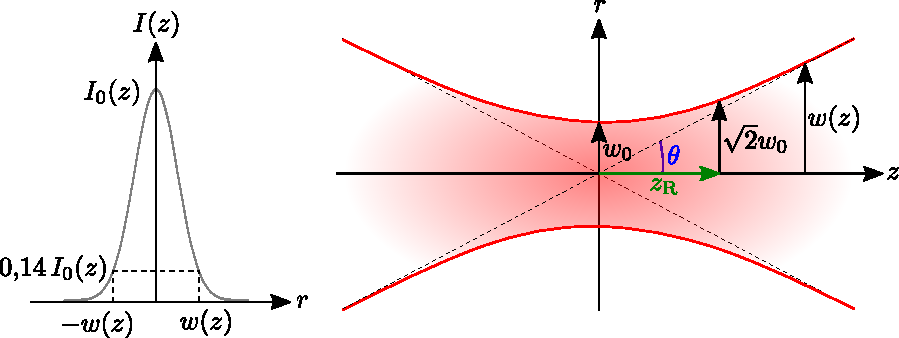
\includegraphics[width=0.9\textwidth]{Figures/faisceau.pdf}
\caption{Paramètres caractéristiques du faisceau laser.}
\label{fig:faisceau}
\end{figure}

Une coupe de l'intensité $I(r,z)$ à $z$ fixé à une allure gaussienne, de largeur typique $w(z)$. À la distance $r=w(z)$, il ne reste plus que \SI{14}{\percent} de l'intensité maximale puisque
\begin{equation}
\frac{I(r=w(z),z)}{I_0(z)}=\e^{-2}\simeq \num{0,14}.
\end{equation}

\subsection{Approximations cylindrique ou conique}
On peut distinguer deux zones pour le faisceau suivant que $z$ est petit ou grand devant la longueur de Rayleigh $z_R$.
\begin{figure}[h!]
\centering
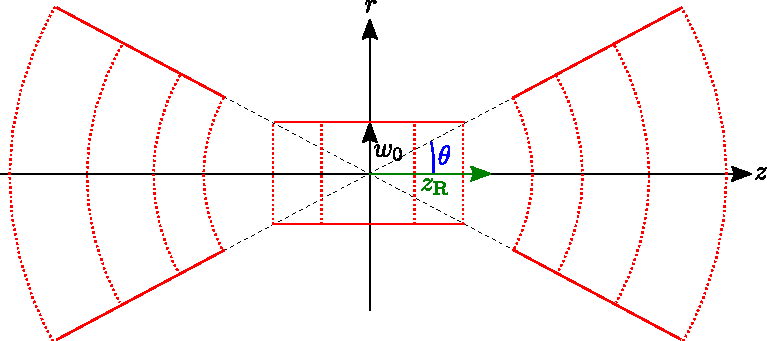
\includegraphics[width=0.8\textwidth]{Figures/cone_cylindre.pdf}
\caption{Modèle cône-cylindre simplifié du faisceau laser. Les surfaces d'onde sont représentées en pointillés.}
\end{figure}
\begin{liste}
\item Si \fbox{$\abs{z}\ll z_{\rm{R}}$}, alors $w(z)\simeq w_0$.
% et $I(r,z) \simeq I_0 e^{-2r^2/w_0}$.
L'intensité ne dépend pas de $z$ et le faisceau est donc \important{cylindrique}. Il possède localement les caractéristiques d'une onde plane.
%, tout en étant d'extension spatiale finie puisque ce régime n'est valable que pour $\abs{z}\ll z_{\rm{R}}$.
\item Si \fbox{$\abs{z}\gg z_{\rm{R}}$}, alors $w(z)\simeq z \frac{w_0}{z_{\rm{R}}}=z\tan\theta \simeq z\theta $, où l'angle $\theta$ est défini par
\begin{equation}\label{eq:theta}
  \theta \simeq \frac{w_0}{z_R} = \frac{\lambda}{\pi w_0}.
\end{equation}
Le faisceau est \imp{conique} d'ouverture angulaire $\theta$. Il possède localement les caractéristiques d'une onde sphérique. On retrouve in comportement similaire à l'évasement d'un faisceau lumineux par \imp{diffraction} qui traverse un obstacle de taille caractéristique $\pi\omega_0$. Autrement dit tout se passe comme si le faisceau cylindrique de rayon $w_0$ était diffracté par son propre bord.
\end{liste}
La longueur de Rayleigh $z_{\rm{R}}$ détermine donc la transition entre l'approximation cylindrique et l'approximation conique du faisceau gaussien.
% divergent d'ouverture angulaire $\theta$.

\begin{exemple}{Ordres de grandeur}
Pour le laser He-Ne utilisé en TP, le col vaut $w_0\simeq\SI{0,3}{mm}$ pour une longueur d'onde $\lambda=\SI{632,8}{nm}$, ce qui donne une longueur de Rayleigh $z_{\rm{R}}=\frac{\pi w_0^2}{\lambda}\simeq \SI{45}{cm}$. L'ouverture angulaire vaut $\theta\simeq\frac{\lambda}{\pi w_0}\simeq \SI{7e-4}{rad}$. Si on place un écran à une distance $D\simeq \SI{2}{m}$,
le faisceau laser prend la forme d'une tâche de diamètre $D \theta \simeq \SI{1,3}{mm}$.

\end{exemple}

\subsection{Focalisation par une lentille}
%Nous allons utiliser le modèle cône-cylindre précédent, en comparant la longueur de Rayleigh $z_{\rm{R}}$ avec la distance focale de la lentille $f'$.
\parag{Modèle gaussien de la focalisation}

\begin{figure}[h!]
\centering

\includegraphics[width=0.75\textwidth]{focalisation.pdf}
\end{figure}

Le modèle du faisceau gaussien permet aussi de corriger les prédictions de l'optique géométrique sur le comportement d'une lentille. En effet, considérons un faisceau parallèle (pas forcément issu d'un laser), dont le profil d'intensité est cylindrique de rayon $w_0$, qui arrive en incidence normale sur une lentille mince convergente, étudiée dans les conditions de Gauss. L'optique géométrique prévoit que le faisceau lumineux converge au point focal image $F'$, puis diverge avec une ouverture angulaire
\begin{equation}
  \theta'\simeq\frac{w_0}{f'}.
\end{equation}

D'après le modèle ondulatoire de la lumière, la diffraction interdit au faisceau de converger rigoureusement en un point. Au lieu de cela, le faisceau atteint un rayon minimal non nul $w_0'$ au point focal image $F'$. En modélisant le faiceau en sortie de la lentille par un faisceau gaussien, on a d'après l'\Eq{theta},
\begin{equation}
  w_0' \simeq \frac{\lambda }{\pi \theta'} \simeq \frac{\lambda f'}{\pi w_0}.
\end{equation}

\begin{theorem}[Rayon minimal d'un faisceau focalisé]\label{form:}
Un faisceau de rayon $w_0$ focalisé par une lentille de focale $f'$ est de rayon minimal
\begin{equation*}
    w_0'\simeq \frac{\lambda f'}{\pi w_0}.
\end{equation*}
\end{theorem}
Le rayon maximal du faisceau incident vérifie $f' \sim \pi w_0 $ en pratique. Ainsi, le rayon minimal du faisceau focalisé est en pratique de l'ordre de la longueur d'onde, $w_0' \sim \lambda$.
On remarque que
 % indique qu'en réalité le faisceau atteint en $F'$ une taille minimale $w_0'$ telle que $\theta'=\frac{\lambda}{\pi w_0'}$.
%
% En égalisant les expressions des angles, il vient finalement que
\begin{equation}
\frac{w_0'}{w_0}=\frac{f'}{z_{\rm{R}}}.
\end{equation}
Comme on cherche à focaliser le faisceau, on veut minimiser $\frac{w_0'}{w_0}$. Il faut donc choisir une lentille de distance focale $f'\ll z_{\rm{R}}$ la plus petite possible.
%L'utilisation d'une lentille de courte focale permet de focaliser un faisceau laser dans son plan focal image. Néanmoins, dans le meilleur des cas on a $f'\simeq w_0$ et donc on en déduit $w_0'\simeq \lambda$.

\parag{Élargisseur de faisceau}
On ajoute maintenant une seconde lentille convergente en sortie dont le foyer objet $F_2$ est confondu avec le foyer image  $F_1'$ de la première lentille. On a alors $F'_1=F_2$ et le système optique est afocal, comme pour une lunette astronomique. On suppose que le faisceau incident est gaussien, de col $w_0$ et d'ouverture angulaire $\theta$ loin en amont de la lentille. De même, le faisceau en sortie est gaussien, de col $w_0''$ et d'ouverture angulaire $\theta''$ loin en aval de la lentille. On souhaite relier les ouvertures angulaires $\theta$ et $\theta''$.

\begin{figure}[h!]
\centering

\includegraphics[width=0.7\textwidth]{élargissement.pdf}
\end{figure}
Pour cela, on applique des formules de trigonométrie au faisceau intermédiaire pour trouver
\begin{equation}
\theta'=\frac{w_0}{f'_{1}}=\frac{w_0''}{f'_{2}}.
\end{equation}
Or $\theta=\frac{\lambda}{\pi w_0}$ et $\theta''=\frac{\lambda}{\pi w_0''}$ sont inversement proportionnels aux cols $w_0$ et $w_0'$, et donc
\begin{equation}
\frac{w_0}{w_0''}=\frac{\theta''}{\theta}=\frac{f'_1}{f'_2} = G,
\end{equation}
où $G$ désigne le grossissement du système optique. Si $f'_2\gg f'_1$, alors $w_0'' \gg w_0$ et on forme un \imp{élargisseur de faisceau}. De plus, $\theta'' \ll \theta$ et donc on réduit la divergence du faisceau.

\begin{definition}[Élargisseur de faisceau]\label{def:}
  Un élargisseur de faisceau est un doublet afocal de lentille tel que $f'_2\gg f'_1$. Les cols des faisceaux gaussiens en entrée et en sortie vérifient
  \begin{equation}
    w_0'' = \frac{f_2'}{f_1'} \,w_0.
  \end{equation}
\end{definition}


\end{document}
